\section{问题分析}

本文的统一主线是“烘房边界驱动内部热质传递，再由全域状态判定烘干是否完成”。问题一的核心是固定圆柱中的非稳态径向传热和含水率扩散；问题二在此基础上引入物性反馈，使温度与含水率形成双向耦合；问题三不改变问题二的物理模型，而是从连续场中寻找最大含水率首次达到阈值的时刻；问题四则同时改变计算区域和物性组，需要处理材料运动、干基守恒以及几何与物性效应的竞争。

问题一中热物性为常数，温度场与水分场在数学上解耦，但扩散率仍随含水率变化。问题二必须从共同初值重新计算，不能将问题一末态作为初态。问题三的“各处均低于阈值”要求采用全域最大值，而不是平均含水率或有限采样点。问题四的半径轨迹由附件给定，材料坐标变换只固定计算域，不能删去收缩造成的 $1/R^2$ 内部尺度和 $1/R$ 表面尺度。

总体求解路线为：输入审计与单位统一、径向环形有限体积离散、内部 Kirchhoff 水分通量和表面 Robin 半控制体求解、自适应 BDF 时间推进、连续场重构与事件定位，最后通过网格、时间容差、输入延拓和四组合对照验证结果。干燥模型分类与连续介质热质传递的选型参考文献[\cite{ref1,ref2}]。

\begin{figure}[H]
  \centering
  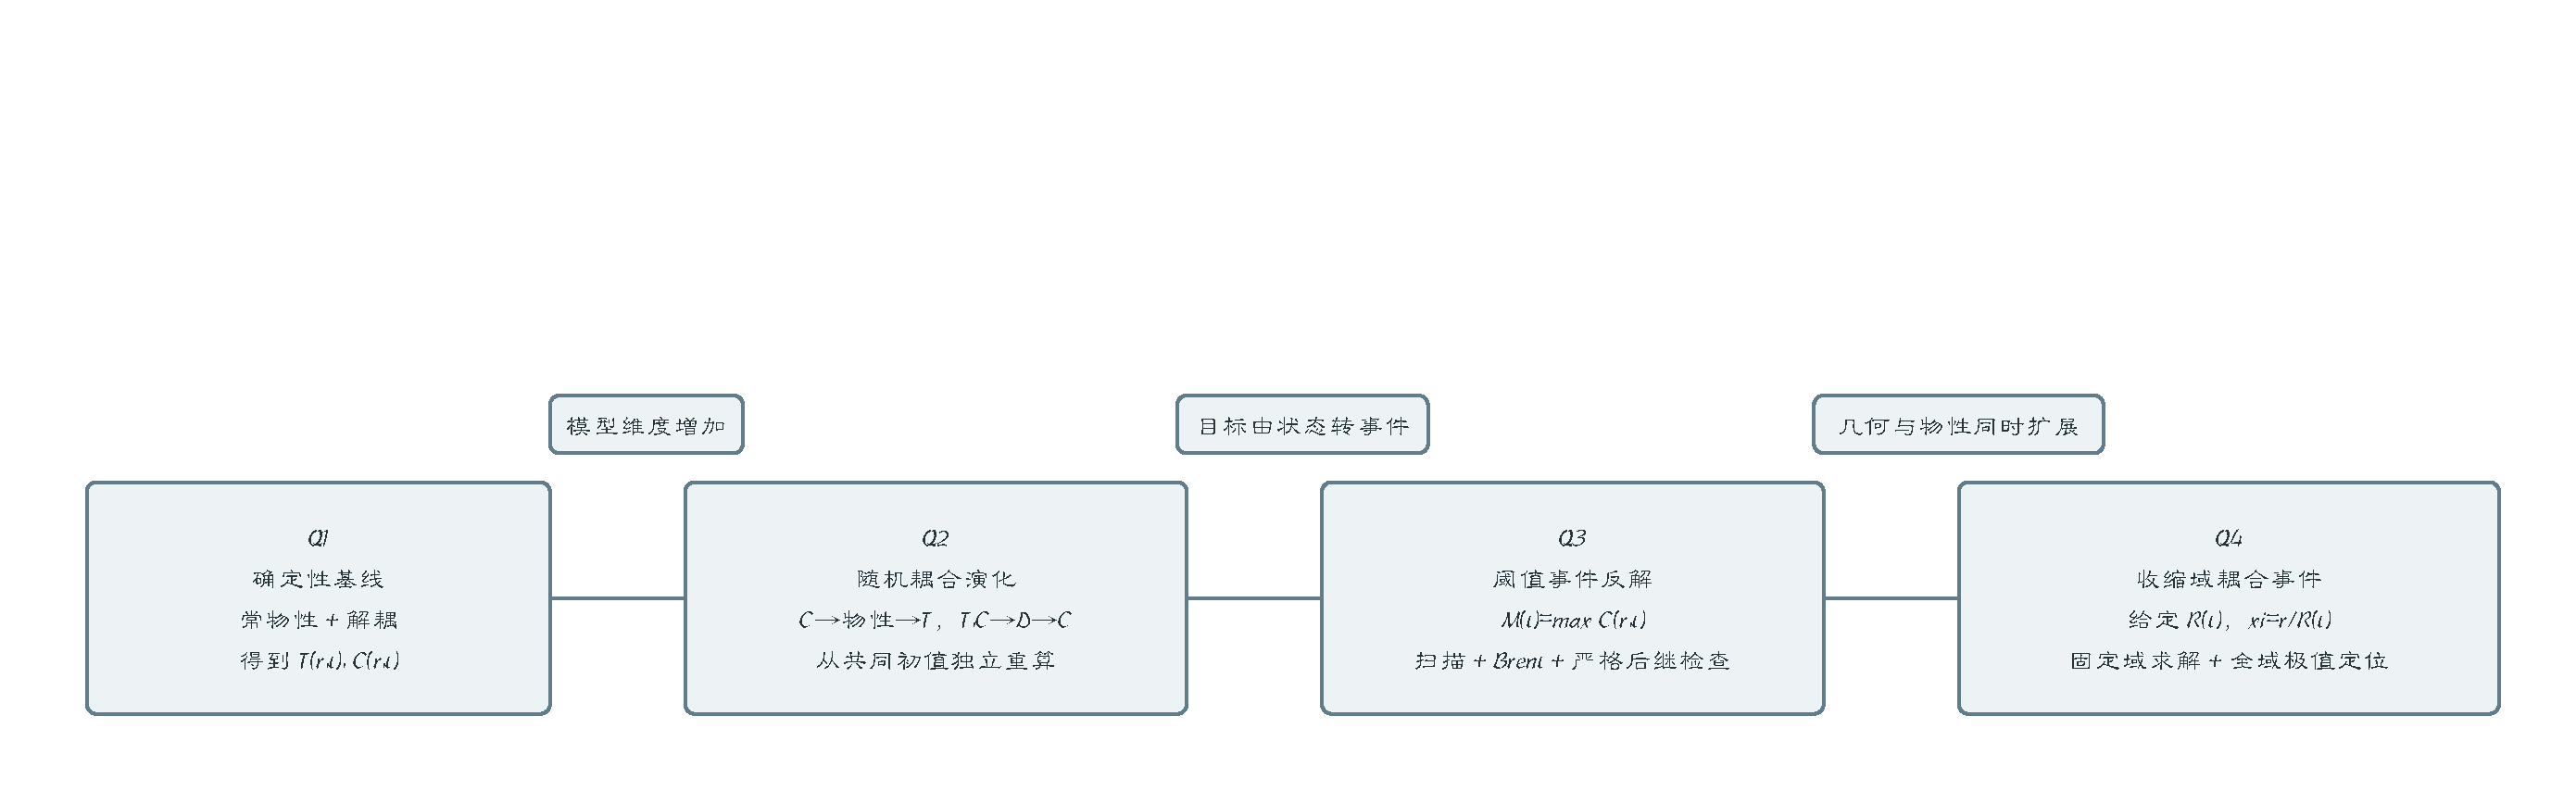
\includegraphics[width=0.92\textwidth]{../figures/fig_question_progression.pdf}
  \caption{四个子问题的递进关系}
  \label{fig:progression}
\end{figure}

图~\ref{fig:progression}用于概括四问之间的模型递进；统一计算和验证闭环见图~\ref{fig:roadmap}。

\begin{figure}[H]
  \centering
  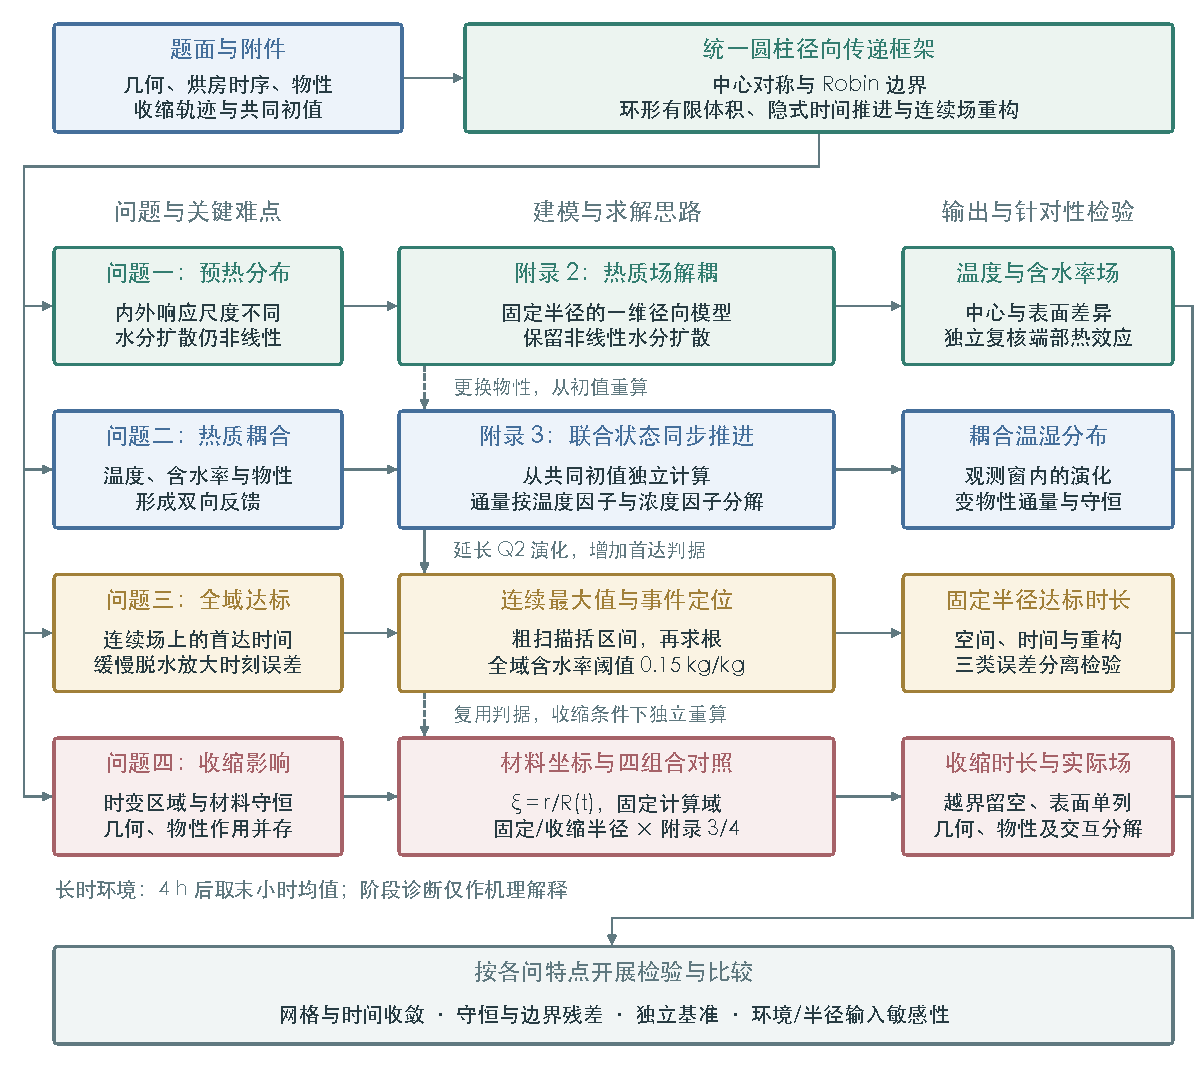
\includegraphics[width=0.92\textwidth]{../figures/fig_roadmap.pdf}
  \caption{本文总体技术路线}
  \label{fig:roadmap}
\end{figure}
